\documentclass{beamer}
\usetheme[bullet=circle,
          titleline=true,
          alternativetitlepage=true,
          titlepagelogo=images/vagrant-bg.png
          ]{Torino}

\usecolortheme{vagrant}

\usepackage{listings}
\usepackage[utf8]{inputenc}
\usepackage[brazilian]{babel}

\author{Jonhnny Weslley \\ @jweslley}
\title{Virtualizando o ambiente de desenvolvimento com Vagrant}
\institute{Gurupi \\ Grupo de Usuários de Ruby do Piauí}
\date{16/Março/2013}

\begin{document}

\begin{frame}[t,plain]
\titlepage
\end{frame}

\begin{frame}[plain,c]
  \begin{center}
    \Huge Virtualização
  \end{center}
\end{frame}

\begin{frame}[plain,c]
  \begin{center}
    \Huge Virtualização
  \end{center}
  \begin{center}
    Motivação
  \end{center}
\end{frame}

\begin{frame}[fragile]{Mundo ideal}
  \begin{verbatim}
  $ git clone git://mycompany.com/dominacao-global.git
  $ run
  \end{verbatim}
\end{frame}

\mode<all>
{\usebackgroundtemplate{
  \vbox to \paperheight{
    \vfil\hbox to \paperwidth{
      \hfil
\includegraphics[width=5cm]{images/trollface.jpg}\hfil
    }\vfil
  }
}
\begin{frame}[plain]
\end{frame}}
\mode<all>{\usebackgroundtemplate{}}
\mode*

\begin{frame}[fragile]{Mundo real}
  \begin{verbatim}
  $ git clone git://mycompany.com/dominacao-global.git

  Ler README...

  $ mkdir, make, apt-get, install, vim, ....

  Google, stackoverflow, ...

  Consulta guru, oraculo, amigo, avó, ...

  ...

  $ run
  \end{verbatim}
\end{frame}

\mode<all>
{\usebackgroundtemplate{
  \vbox to \paperheight{
    \vfil\hbox to \paperwidth{
      \hfil
\includegraphics[width=5cm]{images/trollface-lascou.jpg}\hfil
    }\vfil
  }
}
\begin{frame}[plain]
\end{frame}}
\mode<all>{\usebackgroundtemplate{}}
\mode*

\begin{frame}[plain,c]
  \begin{center}
    \Huge Por que?
  \end{center}
\end{frame}

\mode<all>
{\usebackgroundtemplate{
\includegraphics[width=\paperwidth]
{images/so.jpg}}
\begin{frame}[plain]
\end{frame}}
\mode<all>{\usebackgroundtemplate{}}
\mode*

\begin{frame}[plain,c]
  \begin{center}
    \Huge Solução
  \end{center}
\end{frame}

\mode<all>
{\usebackgroundtemplate{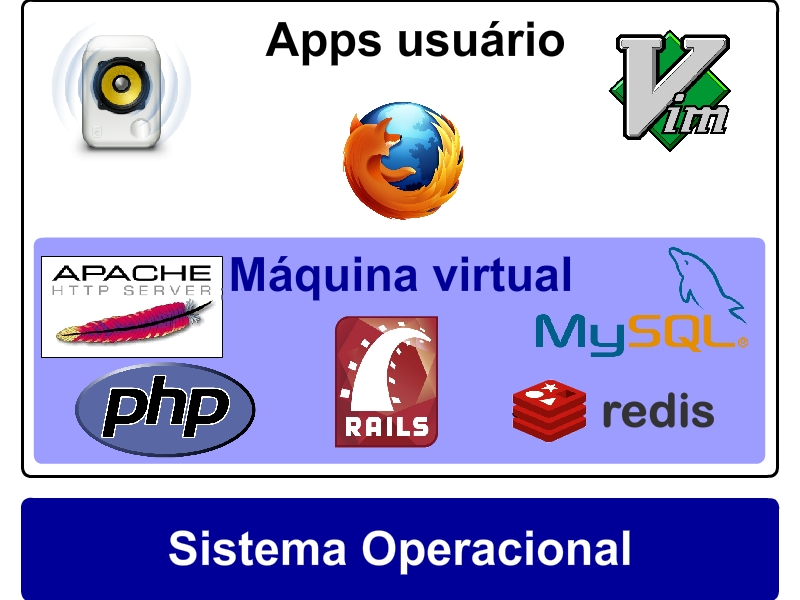
\includegraphics[width=\paperwidth]
{images/vm.jpg}}
\begin{frame}[plain]
\end{frame}}
\mode<all>{\usebackgroundtemplate{}}
\mode*

\begin{frame}[plain,c]
  \begin{center}
    \Huge Vagrant
  \end{center}
  \begin{center}
    Virtualização
  \end{center}
\end{frame}

\begin{frame}[fragile]{Vagrant}
  \begin{itemize}
    \item Mitchell Hashimoto \& John Bender
    \item http://vagrantup.com
    \item Utiliza Virtualbox e Ruby
    \item Funciona em Mac OS, Linux, Windows
  \end{itemize}
\end{frame}

\begin{frame}[fragile]{Vagrant}
  \begin{verbatim}
$ gem install vagrant
$ vagrant box add precise64 http://files.vagrantup.com/precise64.box
$ vagrant init precise64
$ vagrant up
$ vagrant ssh
  \end{verbatim}
\end{frame}

\begin{frame}[plain,c]
  \begin{center}
    \Huge Demonstração
  \end{center}
  \begin{center}
    Comandos e Vagrantfile
  \end{center}
\end{frame}

\begin{frame}{Beneficios - Virtualização/Vagrant}
  \begin{itemize}
    \item Simplicidade
    \item Agilidade
    \item Consistência
    \item Reproducibilidade
    \item Possibilita criar ambiente semelhante ao ambiente de produção
    \item Aumenta produtividade
    \item Descartável
  \end{itemize}
\end{frame}

\begin{frame}{Funcionalidades}
  \begin{itemize}
    \item Boxes
    \item Compartilhamento de arquivos
    \item Port fowarding
    \item Multi-VM
    \item Provisioning/Automatização
    \item Packaging
  \end{itemize}
\end{frame}

\begin{frame}{Boxes}
  \begin{itemize}
    \item Boxes oficiais
    \begin{itemize}
      \item lucid32, lucid64, precise32, precise64
      \item http://files.vagrantup.com/NOME.box
    \end{itemize}
    \item Vagrantbox.es
    \begin{itemize}
      \item http://www.vagrantbox.es/
    \end{itemize}
  \end{itemize}
\end{frame}

\begin{frame}[fragile]{Compartilhamento de arquivos}
  \begin{itemize}
    \item Por padrão o diretório que contém o Vagrantfile é compartilhado em /vagrant
    \item Porém é possivel compartilhar outros diretórios:
  \end{itemize}
  \begin{verbatim}
    config.vm.share_folder 'nome', 'path/guest', 'path/host'
  \end{verbatim}
\end{frame}

\begin{frame}[fragile]{Port fowarding}
  \begin{verbatim}
    # config.vm.forward_port "nome", guestport, hostport
    config.vm.forward_port "http", 80, 9000
    config.vm.forward_port "redis", 6379, 6379
    config.vm.forward_port "mysql", 3306, 3306
  \end{verbatim}
\end{frame}

\begin{frame}[fragile]{Multi-VM}
  \begin{verbatim}
    config.vm.define :web do |web_config|
      web_config.vm.box = "ubuntu"
      web_config.vm.forward_port "http", 80, 8080
      ...
    end
    config.vm.define :db do |db_config|
      db_config.vm.box = "centos-mysql"
      db_config.vm.forward_port "mysql", 3306, 3306
      ...
    end
  \end{verbatim}
\end{frame}

\begin{frame}{Provisioning/Automatização}
  \begin{itemize}
    \item Shell
    \item Chef
    \item Puppet
  \end{itemize}
\end{frame}

\begin{frame}[plain,c]
  \begin{center}
    \Huge Demonstração
  \end{center}
  \begin{center}
    Provisioning
  \end{center}
\end{frame}

\begin{frame}{Provisioning: Chef}
  \begin{itemize}
    \item Tarefas são organizadas em receitas (recipes)
    \item Existem vários livros de receitas (cookbooks)
    \begin{itemize}
      \item http://community.opscode.com/cookbooks
    \end{itemize}
    \item Automatização
    \item Reproducibilidade
  \end{itemize}
\end{frame}


\begin{frame}[plain,c]
  \begin{center}
    \Huge Demonstração
  \end{center}
  \begin{center}
    Chef
  \end{center}
\end{frame}

\mode<all>
{\usebackgroundtemplate{
  \vbox to \paperheight{
    \vfil\hbox to \paperwidth{
      \hfil
\includegraphics[width=5cm]{images/trollface-funfou.jpg}\hfil
    }\vfil
  }
}
\begin{frame}[plain]
\end{frame}}
\mode<all>{\usebackgroundtemplate{}}
\mode*

\begin{frame}{Packaging}
  \begin{itemize}
    \item Criação de boxes customizadas
    \item Diminui tempo de configuração
    \item vagrant package
  \end{itemize}
\end{frame}

\begin{frame}[plain,c]
  \begin{center}
    \Huge Demonstração
  \end{center}
  \begin{center}
    Packaging
  \end{center}
\end{frame}

\begin{frame}[plain,c]
  \begin{center}
    \Huge Dúvidas?
  \end{center}
\end{frame}

\begin{frame}
  \begin{center}
    \Huge Jonhnny Weslley \\ @jweslley
  \end{center}
  \begin{center}
    https://github.com/jweslley/gurupi-vagrant
  \end{center}
\end{frame}

\end{document}
